\section{Программная среда разработки мультиагентных систем и приложений JADE}
\subsection{Общее представление и описание среды}
Java Agent Development Framework (JADE)~--- программная среда разработки мультиагентных систем и приложений, поддерживающая FIPA-стандарты для интеллектуальных агентов. Именно эта реализация технологии программных агентов для платформы Java используется в данном дипломном проекте для разработки распределенной системы.
\begin{figure}[h]
\center{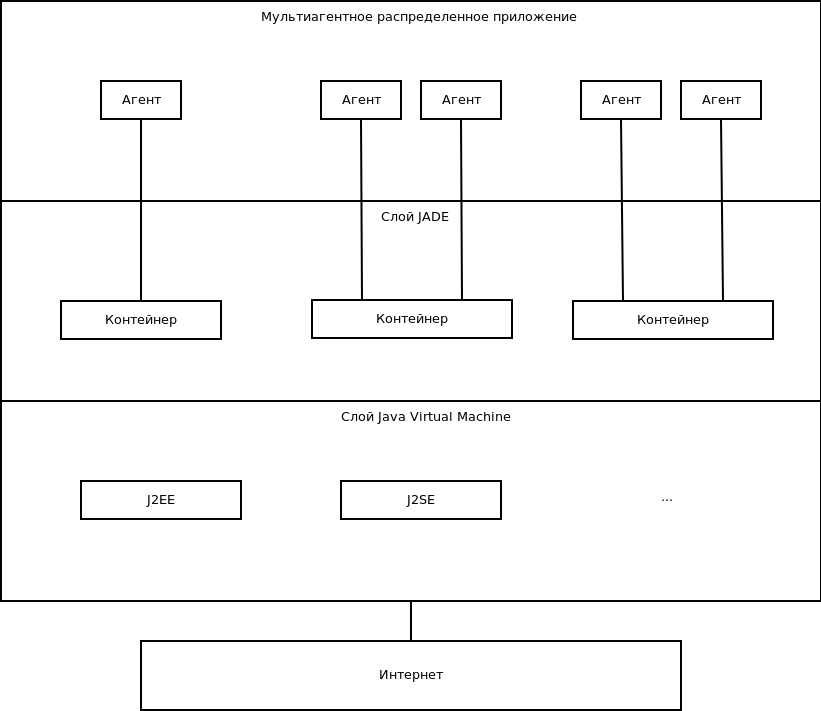
\includegraphics[width=0.8\linewidth]{fipa2}}
\caption{Мультиагентное приложение в рамках JADE}
\label{1:tanenbaum-agent}
\end{figure}

Данная платформа включает в себя:
\begin{itemize}
\item среду выполнения агентов. Агенты регистрируются и работают под управлением среды;
\item библиотеку классов, которые используются для разработки агентных систем;
\item набор графических утилит для администрирования и наблюдения за жизнедеятельностью активных агентов.
\end{itemize}

Программная среда JADE может быть подключена к любому проекту на языке Java.
JADE~--- это программное обеспечение промежуточного слоя, разработанное компанией TILAB, предназначенное для создания распределенных мультиагентных приложений на основе транспортной архитектуры <<точка -- точка>>. И интеллект, и инициатива, и информация, и ресурсы, и контроль могут быть полностью распределены по мобильным терминалам также как и по компьютерам выделенной сети. Среда может динамично взаимодействовать с узлами, которые в терминологии JADE называются агентами. Агенты то появляются, то исчезают в системе в соответствии с потребностями и требованиями программной среды.

Коммуникации между узлами не зависят от типа сети (проводная, беспроводная). Они являются полностью симметричными, и каждый узел может, как инициировать запросы, так и отвечать на них.

Платформа JADE полностью разработана на языке Java. Основополагающие принципы платформы:
\begin{itemize}
\item функциональная совместимость~--- продукт JADE разработан в соответствии со спецификациями FIPA. Как следствие JADE-агенты могут взаимодействовать со сторонними агентами, поддерживающими этот стандарт;
\item портируемость и единообразность~--- продукт JADE предоставляет гомогенный набор прикладных программных интерфейсов(API), которые не зависят ни от базового устройства сети, ни от версии платформы Java. Если подробнее, то в процессе исполнения данное ПО предоставляет одни и те же API для окружений J2EE, J2SE, J2ME. При развертывании разработчики приложений должны определить тип среды исполнения Java;
\item простота использования~--- набор простых и интуитивно-понятных интерфейсов API прячет сложную логику ПО промежуточного слоя от пользователя;
\item принцип <<разрабатывать по средствам>>~--- программистам нет необходимости использовать все возможности, которые предоставляет ПО промежуточного слоя. От программистов не требуется знать что-либо о неиспользуемых функциях платформы. Ни одна из незадействованных функций не создает дополнительные накладные вычислительные расходы.
\end{itemize}

\subsection{Контейнеры и платформы}
На рисунке \ref{2:jade} показаны основные архитектурные элементы платформы JADE.
\begin{figure}[h]
\center{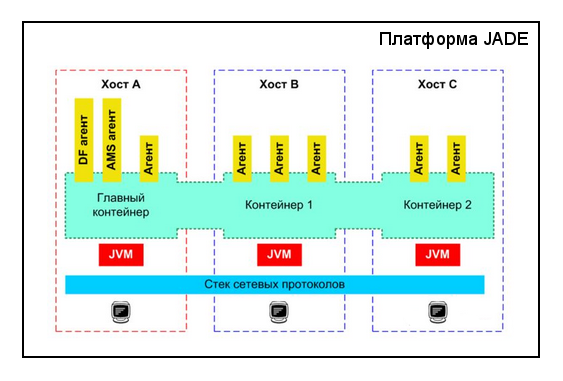
\includegraphics[width=0.9\linewidth]{jade}}
\caption{Составные части платформы JADE}
\label{2:jade}
\end{figure}

Платформа JADE состоит из системы контейнеров, распределенных в сети.
Обычно на каждом хосте находится по одному контейнеру (но для отладочных целей их может быть несколько). Агенты существуют внутри контейнеров, где обеспечиваются описанные выше системные сервисы. В системе может быть только один главный контейнер, который представляет собой точку начальной загрузки платформы. Главный контейнер создается первым, все созданные позже контейнеры должны быть зарегистрированы в главном контейнере.

Главный контейнер хранит набор системных агентов, которые обеспечивают сервисы необходимые для взаимодействия агентов:
\begin{itemize}
\item AMS (Agent Management System)~--- данный агент управляет всей платформой. Этот агент необходим для взаимодействия агентов платформы, он обеспечивает доступ агентов к сервису белых страниц платформы и управляет их жизненным циклом. AMS обеспечивает различные операции платформы, такие как: создание и удаление агентов, удаление контейнеров, завершение работы платформы. Каждому агенту необходимо зарегистрироваться в AMS, для получения персонального идентификатора AID. Запуск агента AMS происходит внутри главного контейнера платформы, но может существовать в любом контейнере. Агент, совершающий действия связанные с функционированием платформы, должен вначале запросить подтверждение у агента AMS;
\item DF (Directory Facilitator)~--- агент обеспечивает регистрацию сервисов и поиск агента по сервису в желтых страницах. Агенты платформы могут подписываться у DF-агента на получение информации о регистрации необходимого сервиса.
\end{itemize}

Внутри каждого контейнера содержится:
GADT (global agent descriptor table)~--- это регистр агентов платформы, в котором хранятся их текущий статус и местоположение.
LADT (local agent descriptor table)~--- тоже самое что и GADT, но для агентов контейнера.

\subsection{Жизненный цикл агента}
В общем случае, жизненный цикл агента включает в себя:
\begin{itemize}
\item создание агента (Agent Creation)~--- исходная точка, с которой начинается существование агента;
\item принятие решения (Making Decision)~--- основное состояние агента;
\item ожидание задания (Waiting for task)~--- состояние пассивного ожидания задания;
\item выполнение задания (Task Execution)~--- активное состояние;
\item возврат результатов (Results Return)~--- передача результатов обработки агенту-инициатору, запросившему выполнение задания;
\item делегирование задания (Delegate)~--- передача всего задания или его части одному или нескольким агентам;
\item ожидание результатов (Waiting for Results)~--- ожидание результатов обработки делегированных задач;
\item клонирование (Clone)~--- создание собственной копии, выполняющейся параллельно оригиналу;
\item перемещение (Move)~--- перемещение собственного тела на другую вычислительную платформу;
\item приостановка (Suspend)~--- временная остановка для экономии ресурсов вычислительной платформы;
\item взаимодействие со средой (Environment Interaction) – запросы к датчикам и мониторинг состояния среды;
\item уничтожение (Terminate)~--- завершающий этап жизненного цикла агента.
\end{itemize}

Такие состояния как перемещение или клонирования используются не всегда: не каждому агенту в процессе своего жизненного цикла потребуются переходы в данные состояния.

Класс Agent обеспечивает открытые методы для перехода из одного состояния в другое; эти методы получили названия от соответствующих переходов в машине конечных состояний:
\begin{itemize}
\item doActivate()~--- переводит агента из состояния AP\_SUSPENDED в состояние AP\_ACTIVE или AP\_WAITING (в зависимости от того состояния, в котором находился агент при вызове doSuspend()). doClone(Location, String) - переводит агента в состояние AP\_COPY из AP\_ACTIVE;
\item doDelete()~--- переводит агента из состояний AP\_SUSPENDED, AP\_WAITING, AP\_ACTIVE в состояние AP DELETED;
\item doMove(Location)~--- переводит агента из состояния AP\_ACTIVE в состояние AP\_TRANSIT;
\item doSuspend()~--- переводит агента из состояний AP\_ACTIVE или AP\_WAITING в состояние AP\_SUSPENDED. Состояние будет сохранено и восстановлено при вызове метода doActivate();
\item doWait(), doWait(long)~--- переводит агента из состояния AP\_ACTIVE в состояние AP\_WAITING;
\item doWake()~--- переводит агента из состояния AP\_WAITING в состояние AP\_ACTIVE.
\end{itemize}

\begin{figure}[h]
\center{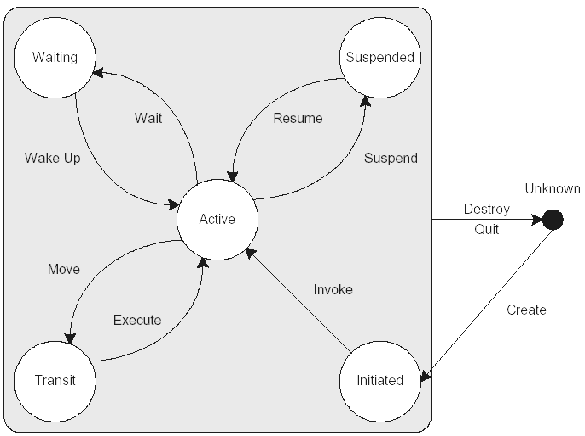
\includegraphics[width=0.8\linewidth]{life-cycle}}
\caption{Диаграмма состояний жизненного цикла агента}
\label{2:life-cycle}
\end{figure}

Агент выполняет поведения (задачи) только в состоянии AP\_ACTIVE. При вызове метода doWait() блокируется целиком весь агент и вся его деятельность, а не выполняемые правила поведения, откуда был произведен вызов данного метода. Для блокирования выполняемого поведения применяется метод block(), который переводит его в спящий режим.

\subsection{Поведение агента}
Для отработки реакции на события агент имеет поведения. Агент может отрабатывать несколько поведений одновременно. Обработка поведений происходит не по приоритетам (как Java потоки), а совместно. Очередность исполнения отдельных простых поведений не гарантируется, для этого нужно использовать поведения специальных типов или синхронизацию.
Поведениям не выделяются отдельные потоки, так как при большом количестве поведений происходит постоянное переключение между ними, а переключение между потоками происходит относительно долго (вызов поведения как метода происходит в среднем в 100 раз быстрее, чем переключение потоков).
\begin{figure}[h!]
\center{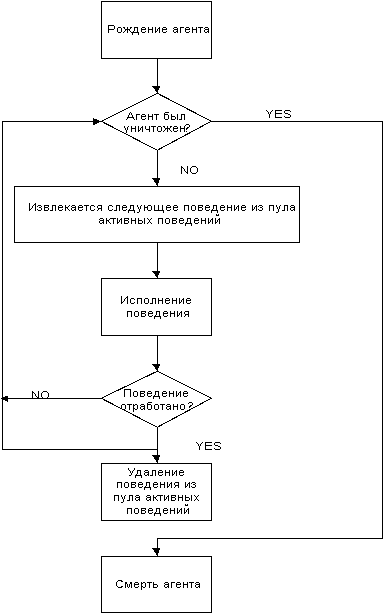
\includegraphics[width=0.6\linewidth]{behs}}
\caption{Алгоритм работы поведений агента}
\label{2:behs}
\end{figure}
В JADE можно выделить три типа поведения.
<<Единоразовое>> поведение. Данный тип поведения завершается сразу, и его метод action() выполняется только один раз. jade.core.behaviours.OneShotBehaviour уже реализовывает метод done(), возвращая true, и может быть удобным образом пронаследован, для реализации данного типа поведения.
\begin{lstlisting}
public class  MyOneShotBehaviour extends OneShotBehaviour { 
   public void action() { 
       // perform operation X 
   } 
 }
\end{lstlisting}
В данном примере операция X выполнится один раз.

<<Циклическое>> поведение никогда не завершается, и его метод action() выполняет одни и те же операции при каждом вызове. jade.core.behaviours.CyclicBehaviour уже реализовывает метод done(), всегда возвращая false, и может быть пронаследован для реализации циклических моделей поведения.
\begin{lstlisting}
public class  MyCyclicBehaviour extends CyclicBehaviour { 
   public void action() { 
       // perform operation Y 
   } 
}
\end{lstlisting}
Операция Y будет выполняться в цикле бесконечно (пока агент, имеющий это поведение, не будет завершен).

Общий случай поведения включает в себя статус, в зависимости от которого выполняются различные операции. Выполнение действий завершается, когда встречается данное условие.
\begin{lstlisting}
public  class MyThreeStepBehaviour extends Behaviour { 
   private int step = 0; 
   public void action() { 
       switch (step) { 
           case 0: 
           // perform operation X 
           step++; 
           break; 
           case 1: 
           // perform operation Y 
           step++; 
           break; 
           case 2: 
           // perform operation Z 
           step++; 
           break; 
       } 
    } 

    public boolean done() { 
        return step == 3; 
    } 
}
\end{lstlisting}

Jade предоставляет возможность соединять простые формы поведения для создания более сложных (SequentialBehaviour, ParallelBehaviour и FSMBehaviour). Помимо этого, Jade содержит два готовых класса (в пакете jade.core.behaviours), с помощью которых можно легко реализовать поведение, позволяющее выполнять определенные действия в заданные моменты времени.
\begin{itemize}
\item WakerBehaviour, в котором методы action() и done() уже реализованы таким образом, что вызывается абстрактный метод handleElapsedTimeout() после того, как истечет заданный промежутка времени (указанный в конструкторе);
\begin{lstlisting}
public class  MyAgent extends Agent { 
   protected void setup() { 
       addBehaviour(new WakerBehaviour(this,  10000) { 
           protected void handleElapsedTimeout() { 
               // perform operation X 
           } 
       }); 
   } 
}
\end{lstlisting}
В данном случае операция X выполнится через 10 секунд после того, как будет выведена надпись <<Adding waker behaviour>>.
\item В TickerBehaviour методы action() и done() реализованы таким образом, что вызывают циклически абстрактный метод onTick(), ожидая некоторое (заданное в конструкторе) время после каждого выполнения. TickerBehaviour никогда не завершится. 
\begin{lstlisting}
public class  MyAgent extends Agent { 
   protected void setup() { 
       addBehaviour(new TickerBehaviour(this,  10000) { 
           protected void onTick() { 
               // perform operation Y 
           } 
       }); 
   } 
}
\end{lstlisting}
Операция Y будет выполняться с периодом в 10 секунд.
\end{itemize}

\subsection{Коммуникационные модели, язык ACL}
Коммуникационная модель, определяет то, каким образом удаленные части программы совместно работают над запросом пользователя. Наиболее распространенным подходом здесь считается пересылка сообщений, позволяющая достичь более высокой степени автономности между частями программы, чем если бы они вызывались директивно посредством RPC (Удаленного Запуска Процедур). Пересылка сообщений является концепцией, естественно подходящей агентным системам, поскольку в рамках нее агент становится достаточно независимой единицей, выполняющей исключительно свои операции, и лишь иногда отвечающей на запросы других агентов или самостоятельно осуществляющей запросы, если это потребуется для ее работы. В рамках этой концепции были выделены следующие модели коммуникации между агентами:
\begin{itemize}
\item синхронная коммуникация. Обычно, когда клиент запускает метод на сервере, сервер выполняет запрошенный метод и возвращает результат клиенту, который продолжает свою работу. Этот стиль называется синхронным, потому что клиент блокируется до тех пор, пока результаты метода не будут возвращены;
\item асинхронная коммуникация. При использовании асинхронной коммуникации клиенту нет необходимости ждать, пока сервер выполнит метод, вместо этого клиент продолжает выполнять свою собственную задачу. В таком случае у клиента есть несколько возможностей получить результаты запущенного метода. Он может периодически опрашивать сервер о том, было ли закончено выполнение метода, он может ждать результата в тех случаях, когда это нужно или подписаться на уведомление о том, что результат будет доступен;
\item динамическая коммуникация. Этот механизм удобен в том случае, когда у клиента нет доступа к прокси серверу. Клиент может сконструировать сообщение динамически, путем указания сигнатуры того серверного метода, который должен быть запущен. Динамическая генерация сообщений может быть использована как синхронно, так и асинхронно;
\item многосвязная коммуникация. Многосвязная коммуникация позволяет клиентам использовать параллелизм в процессе общения с серверными объектами. Используя механизм многосвязной коммуникации, клиент может запускать один и тот же метод на нескольких серверах параллельно.
\end{itemize}

Современная система доступа к распределенным информационным ресурсам, работающая в онлайн-режиме в Internet, должна быть готова к приему и обработке нескольких различных запросов одновременно, поэтому нельзя допустить, чтобы прохождение запросов задерживалось, пока такая система обрабатывает другой запрос. Поэтому коммуникацию между системными агентами в такой распределенной системе целесообразно организовывать по асинхронному принципу, с ориентацией на создание многопоточных программ. Однако, при создании агентов, отвечающих за работу с конечным пользователем системы, могут быть применены разные подходы.

Сервис обмена сообщениями одна из основополагающих частей архитектуры платформы JADE. Сервис основан на асинхронной передаче сообщений. Каждый агент имеет свой <<почтовый ящик>>~--- очередь входящих сообщений, куда помещаются все направленные агенту сообщения. В тот момент, когда сообщение помещается в очередь входящих сообщений, агент оповещается об этом.
\begin{figure}[h]
\center{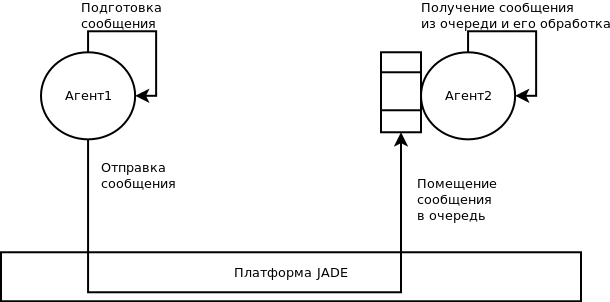
\includegraphics[width=0.6\linewidth]{acl}}
\caption{Межагентное взаимодействие в рамках платформы JADE}
\label{2:acl}
\end{figure}
Сообщения, которыми обмениваются JADE агенты, имеют языковой формат ACL, определенный FIPA. Этот формат сообщения включает в себя несколько обязательных полей и, в частности:
\begin{itemize}
\item отправитель сообщения;
\item список получателей;
\item цель общения (также называемая <<Перформативом>>), указывающая на то, что отправитель намерен достичь путем отправки сообщения. Целевыми сообщениями могут быть REQUEST (запрос), если отправитель желает, чтобы получатель совершил определенное действие, INFORM (информирование), если отправитель желает, чтобы получатель знал о некотором факте, QUERY\_IF (условный запрос), если отправитель хочет знать сохраняются ли данные условия, CFP, PROPOSE(предложение), ACCEPT\_PROPOSAL(принятие предложения), REJECT\_PROPOSAL(отмена предложения), если отправитель и получатель участвуют в переговорах, и многое другое; 
\item содержание т.е. фактическая информация, содержащаяся в сообщении (т.е. действия, которые будут выполняться в REQUEST сообщении, то, что отправитель желает раскрыть в INFORM сообщение ...);
\item язык содержания, т.е. какой синтаксис используется, чтобы выразить содержание (как отправителю, так и получателю необходимо иметь возможность кодировать / раскодировать выражения);
\item онтология, то есть словарь символов, используемых в их содержании и их значения(как отправитель так и получатель должны приписывать тот же смысл символам в сообщении, чтобы корректно понимать его);
\item некоторые поля, используемые для контроля нескольких одновременных разговоров и указания таймаутов для получения ответов, таких, как conversation-ID, reply-with, in-reply-to, reply-by. 
\end{itemize}

С сообщением в JADE работают как с объектом класса jade.lang.acl.ACLMessage, который имеет get и set методы обработки всех полей сообщения.

В случае межплатформенного сценария взаимодействие осуществляется по ACC (Agent Communication Channel). Контейнеры могут быть запущены с различными типами MTP, при этом ACC должен обеспечивать взаимодействие между ними.
В связи с тем, что агенты, обменивающиеся сообщениями, могут находиться как в одном, так и в разных контейнерах JADE использует два типа протокола: MTP (message transport protocol) и IMTP (internal message transport protocol).

В том случае если агенты находятся в разных контейнерах, используется RMI (Java Remote Method Invocation).

В JADE доступны различные типы протоколов MTP, такие как:
\begin{itemize}
\item CORBA IIOP MTP, основанный на стандартном Sun ORB;
\item CORBA IIOP MTP, основанный на ORBACUS и HTTP.
\end{itemize}
